\documentclass[a4paper,11pt]{article}
\usepackage[T1]{fontenc}
\usepackage{color}
\usepackage{amssymb}
\usepackage{amsmath}
\usepackage[dvipsnames]{xcolor}
\usepackage{tikz}
\usetikzlibrary{positioning, calc}
\usetikzlibrary{calc}
\usetikzlibrary{arrows}
\usepackage{tikz-3dplot}
\usetikzlibrary{fadings}
\usetikzlibrary{decorations.pathreplacing,decorations.markings,decorations.pathmorphing}
\tikzset{snake it/.style={decorate, decoration=snake}}
\usetikzlibrary{patterns,patterns.meta}
\usetikzlibrary{decorations}
\tikzset{
	%Define standard arrow tip
    >=stealth',
    %Define style for boxes
    punkt/.style={
           rectangle,
           rounded corners,
           draw=black, very thick,
           text width=6.5em,
           minimum height=2em,
           text centered},
    % Define arrow style
    pil/.style={
           ->,
           thick,
           shorten <=2pt,
           shorten >=2pt,},
    % style to apply some styles to each segment of a path
  on each segment/.style={
    decorate,
    decoration={
      show path construction,
      moveto code={},
      lineto code={
        \path[#1]
        (\tikzinputsegmentfirst) -- (\tikzinputsegmentlast);
      },
      curveto code={
        \path[#1] (\tikzinputsegmentfirst)
        .. controls
        (\tikzinputsegmentsupporta) and (\tikzinputsegmentsupportb)
        ..
        (\tikzinputsegmentlast);
      },
      closepath code={
        \path[#1]
        (\tikzinputsegmentfirst) -- (\tikzinputsegmentlast);
      },
    },
  },
  % style to add an arrow in the middle of a path
  mid arrow/.style={postaction={decorate,decoration={
        markings,
        mark=at position .5 with {\arrow[#1]{stealth'}}
      }}}
}

\begin{document}

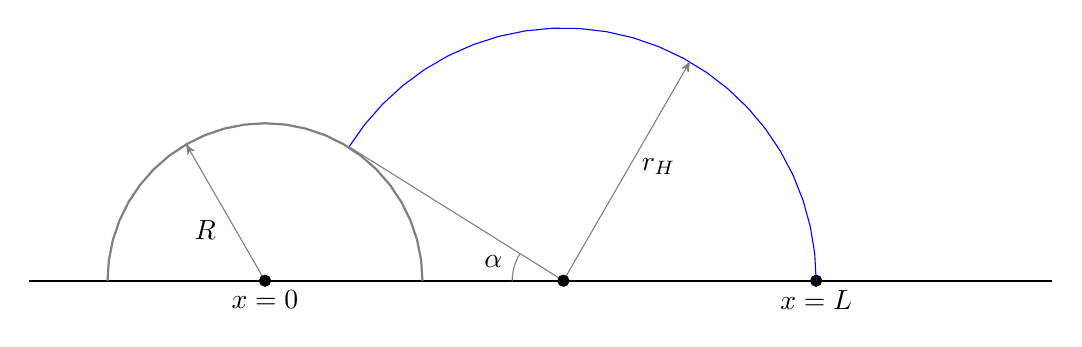
\begin{tikzpicture}[scale=1]

    \draw[gray,->] (0,0) -- ({2*cos(120)}, {2*sin(120)});
    \node[left] at (-0.5,0.65) {$R$};
    
    \draw[thick] (-3,0) -- (10,0);
    \draw [domain=0:180,gray,thick] plot ({2*cos(\x)}, {2*sin(\x)});
    \draw[black] plot [mark=*, mark size=2] coordinates{(0,0)};
    \node[below] at (0,0) {$x=0$};
    
    \draw[black] plot [mark=*, mark size=2] coordinates{(7,0)};
    \node[below] at (7,0) {$x=L$};
    
    \draw [domain=0:148,blue] plot ({3.21*cos(\x)+7-3.21}, {3.21*sin(\x)});
    
    \draw [domain=180:148,gray] plot ({0.65*cos(\x)+7-3.21}, {0.65*sin(\x)});
    \node at (2.9,0.25) {$\alpha$};
    
    \draw[gray,->] ({7-3.21},0) -- ({3.21*cos(60)+7-3.21}, {3.21*sin(60)});
    \node at (5,1.45) {$r_H$};

    \draw[gray] ({7-3.21},0) -- ({3.21*cos(148)+7-3.21}, {3.21*sin(148)});
    \draw[black] plot [mark=*, mark size=2] coordinates{({7-3.21},0)};
    
    \end{tikzpicture}

\end{document}